\todo[inline]{Indsæt kilder}
This section covers the problem domain analysis based on data gathering in form of the initial interview with Ipsen, see section x.
The following subsections include the choice of the selected classes and events, the explanation of the structure between classes, and the description of the behavior patterns through state-chart diagram.

\section{Classes and events}
The following subsections explore the potential class and event candidates as well as the thought process behind it.
The generated class and event candidates will be systematic selected to represent the problem domain with regard to relevance and that they satisfy the system definition.
The process of systematically select classes and events are based on the following criteria found in Object Oriented Design \& Analysis (OOA)\&D \citep[p.~63-67]{Rod-Aalborg} .
\todo[inline]{Kilden skal nok formeteres andreledes, men jeg ved ikke helt hvordan}

\subsection{Classes}
According to OOA\&D a class is defined as:
“A description of a collection of objects sharing structure, behavioral pattern, and attributes.”
% Henrik: Måske lav det til en definition med \begin{defn}noget tekst her\end{defn}
% se hvordan Anna har gjort i PACT analyse afsnit - men hvor?

The questions below help to evaluate a class if those are affirmative. \citep[p.~62]{Rod-Aalborg}
\begin{itemize}
	\item Can you identify objects from the class?
	\item Does the class contain unique information?
	\item Does the class encompass multiple objects?
	\item Does the class have a suitable and manageable number of events?
\end{itemize}
%(citerer direkte fra bogen - er det ok?)

\subsubsection{Class candidates} 
\begin{tabular}{l l}
	\texttt{Company} & A class representing the companies managed by the system \\
	\texttt{Handbook} & A class representing all the documents with the newest version\\
	\texttt{Document} & A class representing the documents\\
	\texttt{User }& A class representing reader, writer and administrator role\\
	\texttt{Version} & A class representing a document’s version and the validity period\\
	\texttt{Log} & A class representing descriptions of changes for each version\\ 
	\texttt{Responsibility} & A class representing the difference user access levels to the handbook\\ 
	\texttt{Approval} & A class representing the created approvals, keeping track of who has been\\&assign to approve what document and version\\ 
	\texttt{TOC} & A class represents the table of contents of the documents in the handbook\\
	\texttt{Notification} & A class to represent which user is assign to which document and send\\&notification to inform there is a new version\\ 
	\texttt{Read Status} & A class that keeps track of who has read which document and version\\
	\texttt{Supplier} & A class describing a supplier, which has to be approved 
\end{tabular}

\subsubsection{Qualifying classes}
The following section covers an explanation whether the generates classes are qualified or not qualified.

The \texttt{Company} class is qualified because it keeps track of companies that use the system, which is an important concept to keep track of.

The \texttt{Handbook} class is qualified for the reason that it keeps track of the documents and is an important part of the problem domain and system definition.

The \texttt{Document} class is qualified because it works as an item for the various versions in an item-descriptor pattern.

The \texttt{Version} class is qualified since it encapsulates the version data in the documents, and allows the document to have multiple instances of them.

The \texttt{User} class is qualified because there would be different types of users with different access levels in the system.

The \texttt{Log} class is not qualified because the class does not contain unique information and the class it self is too simple.
It is unnecessary to create an independent class for the changelog and therefore it has been converted to an attribute for the \texttt{Version} class.

The \texttt{Responsibility} class is not qualified because the different levels of access and permissions are present in the \texttt{User} class.

The \texttt{Approval} class is qualified since it is vital to substantiate who is going to or had approval each version and what date it has been approved.

The \texttt{TOC} class is not qualified since \texttt{TOC} is a property of the \texttt{Handbook} class and does not contains unique information.
The purpose with \texttt{TOC} is to create an overview of the valid documents in the handbook.

The \texttt{Notification} class is not qualified as the notification is more an event rather than a class.
The functionality in the \texttt{Notification} class is to assign users to specific documents therefore the name is modified to \texttt{Department} instead.

The \texttt{Read Status} class is qualified since the system needs to store information regarding what associated user has read what associated version and when.
This is useful when the company has to report a total number of employees that have read the current version of the document.

The \texttt{Supplier} class is qualified seeing that the administrator need to keep a record of all documents related to approval of suppliers. 

Qualified classes:
\begin{itemize} 
	\item \texttt{Company}
	\item \texttt{Handbook}
	\item \texttt{Document}
	\item \texttt{Version}
	\item \texttt{User}
	\item \texttt{Approval}
	\item \texttt{Department}
	\item \texttt{Read Status}
	\item \texttt{Supplier}
\end{itemize}

\subsection{Events}

According to OOA\&D an event is defined as\citep[p.~53]{Rod-Aalborg}:

``An instantaneous incident involving one or more objects.''
% Henrik: Måske også lav dette til en definition med \begin{defn}

Once again the questions below help to evaluate an event if those are affirmative\citep[p.~65]{Rod-Aalborg}.
\begin{itemize}
	\item Is the event instantaneous?
	\item Is the event atomic?
	\item Can the event be identified when it happens?
\end{itemize}

\subsubsection{Event candidates}
\textbf{Document added} - when a document is created\\
\textbf{Document updated} - when an existing document's information is updated\\
\textbf{Document archived} - when a document is not relevant for a company at the present time and need be removed from the handbook\\
\textbf{Document reactivated} - when a document is relevant for the company once again and need to be accessible in the handbook\\
\textbf{Document deleted} - when a retention period has expired for an archived document then it will be possible to delete the document in the system or an administrator accidentally created incorrect content document in the system\\
\textbf{Version approved}  - when a version has been approved\\ 
\textbf{New version released} - when a new version has been approved and the system ensure that it is available in the handbook\\
\textbf{Version archived} - when a handbook contains a new approved version then the system need to ensure that a previous version is archived\\
\textbf{Version marked as read} - when a user has verified that the newest version has been read\\
\textbf{User added} - when an administrator created a user\\
\textbf{User updated} - when an administrator updated a user's information\\
\textbf{User deactivated} - when an administrator removed a user's accessibility for the handbook for instance if that user no longer work for the company\\
\textbf{User reactivated} - when an administrator give a deactivated user access to a handbook\\
\textbf{User deleted} - when an administrator removed a user from the system\\
\textbf{Supplier added} - when a new supplier has been registered in the system\\
\textbf{Supplier updated} - when an existing supplier's information has been updated\\
\textbf{Supplier deleted} - when a supplier has been removed from the system\\
\textbf{Supplier approved} - when a supplier's document has been approved\\
\textbf{Approval requested} - when a new version is created and the approval requested is sent to other users (approver) in the system\\
\textbf{Approval confirmed} - when an approval is rejected by one approver\\
\textbf{Approval denied} - when an approval is confirmed by every approver\\
\textbf{Department added} - when a department is created\\
\textbf{Department updated} - when an existing department's information is updated\\
\textbf{Department deleted} - when an existing department is removed from system\\
\textbf{Document added to department} - when associated a document to a department. This way a department will only have access to relevant documents\\
\textbf{Document removed from department} - when a associate document is removed from a department which means the department no longer have access to the document\\
\textbf{Department notified user} - when a associated user received a notification when a new version is released\\ 
\textbf{Document printed} - when a document is printed\\

\subsubsection{Qualifying events}
In this section the generated events will be reviewed and determined whether they are qualified or not qualified.
The selection and deselection of these candidates will be explained, and the event table will be displayed afterwards.

\textbf{Document added} event is qualified reasoned that a document object must be created first before it has a version object added. 

\textbf{Document updated} event is not qualified since it is a version that are updated which is the same as \textbf{new version released}  event.

\textbf{Document archived} event is qualified because it is an important functionality to archive expired documents for number of years according to ISO 9001 document management requirements. 

\textbf{Document reactivated} event is qualified since if the system can  archive a document, it must also be able to reactivated and make it available in the handbook again. 

\textbf{Document deleted} is qualified for the reason that if an administrator made a mistake and added a wrong document then the delete option is useful. 

\textbf{Version approved} and \textbf{new version released} events are qualified since it is important for the system to registered and keep track of the whether a document is complete with the approval process and whether it should be accessible in the handbook. 

\textbf{Version marked as read} event is qualified because it is crucial for the company register if employees had read and are up to date with the current standards. 

\textbf{Version archived} event is qualified for the same reason as \textbf{document archived} event.

\textbf{User added}, \textbf{user updated}, \textbf{user deactivated}, \textbf{user reactivated} and \textbf{user deleted} events are all qualified as an administrator need to manage company's user list. 

\textbf{Supplier added}, \textbf{supplier updated},  \textbf{supplier deleted} and \textbf{supplier approved} events are all qualified since suppliers need to be manage by an administrator whether they are approved or when to be reapproved. 

\textbf{Approval requested}, \textbf{approval denied}, \textbf{approval confirmed} events are all qualified seeing that it is important part of the system definition that the system must support an approval process before release a new version in the handbook. 

\textbf{Department added}, \textbf{department updated}, \textbf{department deleted} events are qualified since through department will it be possible to associated a specific department to those relevant documents. 

\textbf{Document added to department}, \textbf{document removed from department}, \textbf{department notified user} events are qualified seeing that the system must be able to send notification to the correct user from a specific department that a associated document has released a new version. 

\textbf{Document printed} event is not qualified since the problem domain does not include controlling of printed documents.

Qualified events:
\begin{itemize} 
	\item Document added
	\item Document archived
	\item Document reactivated
	\item Document deleted
	\item Version approved
	\item New version released
	\item Version marked as read
	\item Version archived
	\item User added
	\item User updated
	\item User deactivated
	\item User deleted
	\item Supplier added
	\item Supplier updated
	\item Supplier deleted
	\item Supplier approved
	\item Approval requested
	\item Approval denied
	\item Approval confirmed
	\item Department added
	\item Department updated
	\item Department deleted
	\item Document added to department
	\item Document removed from department
	\item Department notified user
\end{itemize}

\section{Event table}
The result of the selected qualified events and classes is an event table representing their relations. An event that can occur up to one time indicates with a plus symbol +, and an event that can occur multiple times indicates with star symbol *.

\begin{figure}[H]
	\centering
	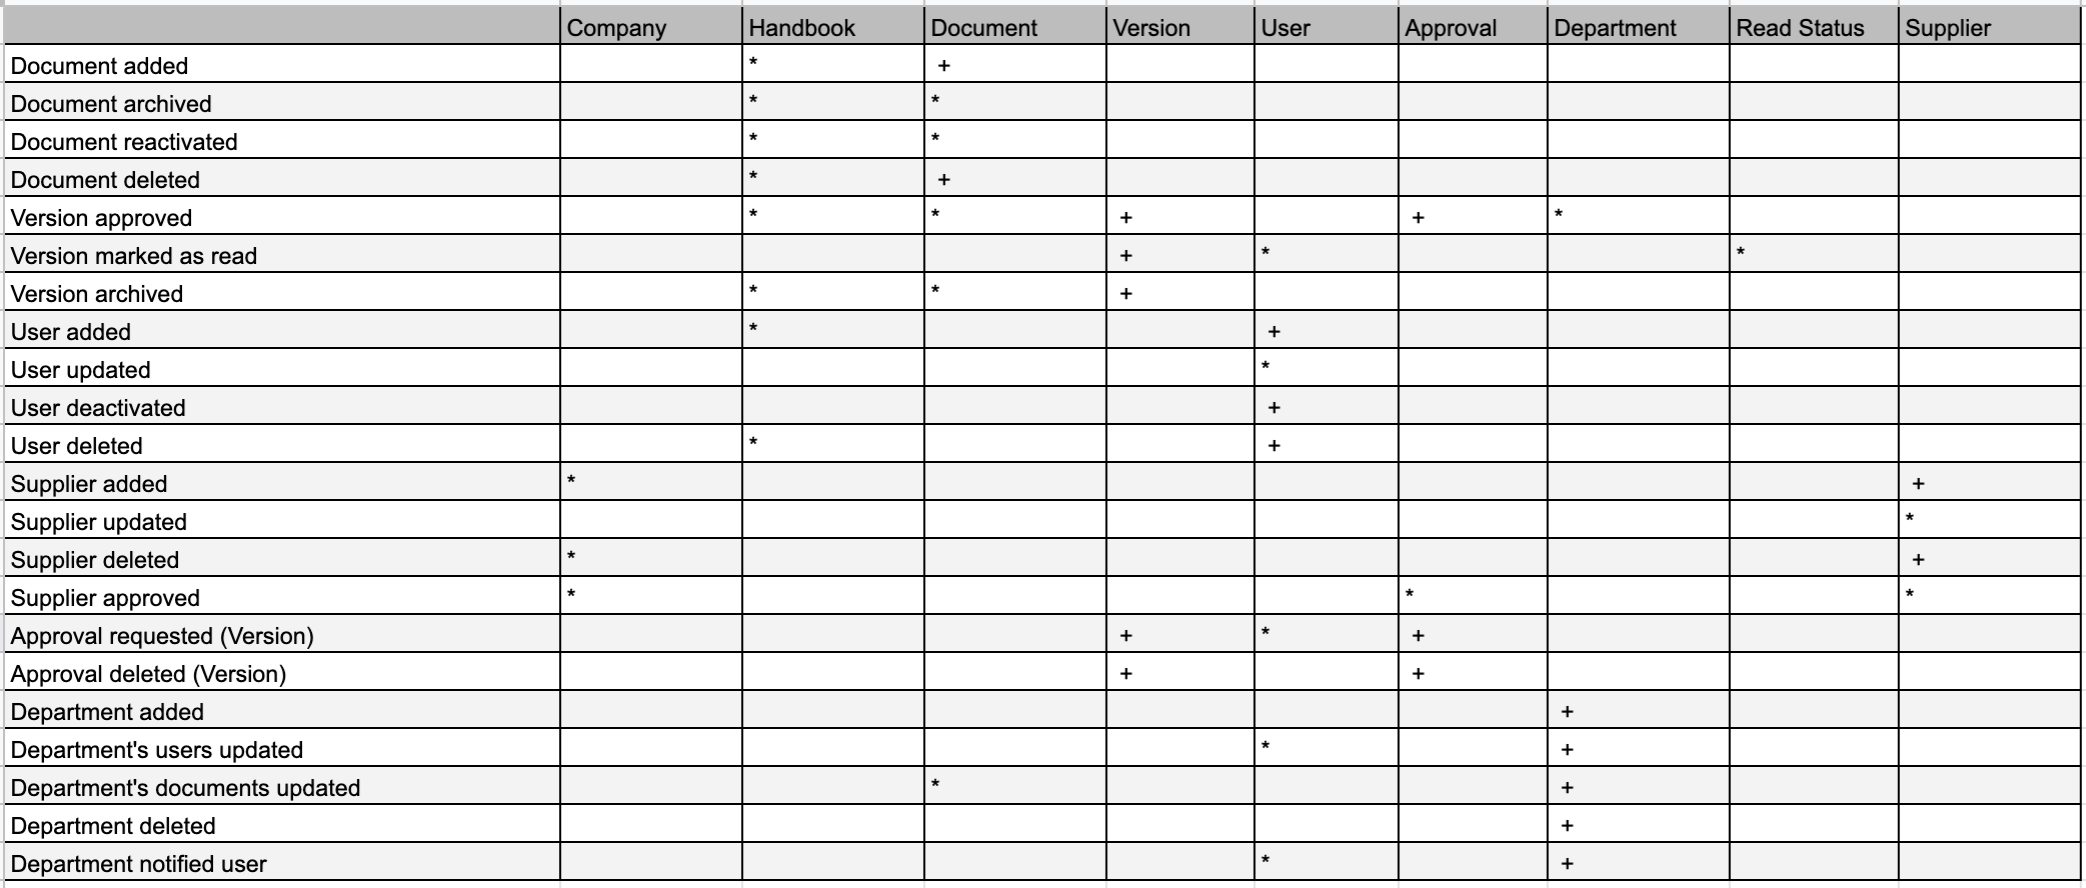
\includegraphics[width=0.95\textwidth]{billeder/Event_table.png}
	\caption{\textit{Event table
	}\label{fig:ClassDiagram}}
\end{figure}

% ændre figure til tabel.. how?

